%!TEX root = volumeFinal.tex 
\chapter{\label{chap:busca}Busca}

Técnicas de busca visam encontrar sequências de ações para um agente alcançar um objetivo.
Para utilizar as técnicas de busca é preciso formalizar o problema a ser resolvido e o objetivo a ser alcançado.
Para isso, é preciso ter um problema e como resolução é retornado um conjunto de ações.
Um problema pode ser definido por cinco componentes~\cite[Capítulo 3]{intelligence2003modern}: 

\begin{itemize}
	\item $s_{0}$, o estado inicial, onde o agente inicia no ambiente;
	\item Ações, conjunto das possíveis ações disponíveis no agente;
	\item $resultado(s, a)$, um modelo de transição, que define o estado resultante após a execução da ação $a$ no estado $s$;
	\item $objetivo(s)$, uma função que verifica se o estado $s$ satisfaz o objetivo do agente e; 
	\item Custo do caminho, uma função que define um valor numérico para cada ação realizada em um estado. O custo é definido dependendo do ambiente, pois o custo pode ser tanto a distancia entre duas localidades, ou o custo monetário de se locomover. 
\end{itemize}   

Tais elementos são necessários como entrada para as técnicas de busca.
A solução é obtida quando o agente iniciando no estado inicial do ambiente $s_{0}$ utiliza o modelo de transição $resultado(s, a)$, através das ações aplicadas nos estados, para chegar a um estado onde satisfaça o objetivo do agente $objetivo(s)$.
Existem diferentes estratégias de busca para encontrar uma solução.
As diferentes técnicas podem encontrar caminhos diferentes para o mesmo problema, isso vem do fato de que o custo do caminho, quando levado em consideração, pode encontrar uma solução ótima, o que significa que a sequência de ações encontrada é a que tem o menor custo de caminho entre todas as soluções~\cite[Capítulo 3]{intelligence2003modern}.

Considere o mapa apresentado na Figura~\ref{fig:mapabusca} para exemplificar um problema de busca.
Cada círculo representa uma cidade, e as linhas entre as cidades são estradas que as ligam umas as outras. 
A ação possível neste problema é a de se locomover entre as cidades que tenham ligação.
O estado inicial é a cidade de São Jerônimo. O resultado do modelo de transição, é a cidade resultante após se locomover. O objetivo do agente é chegar na cidade de Porto Alegre e o custo de cada ação é o valor definido em cima de cada transição. 

\begin{figure}[ht]
	\centering
	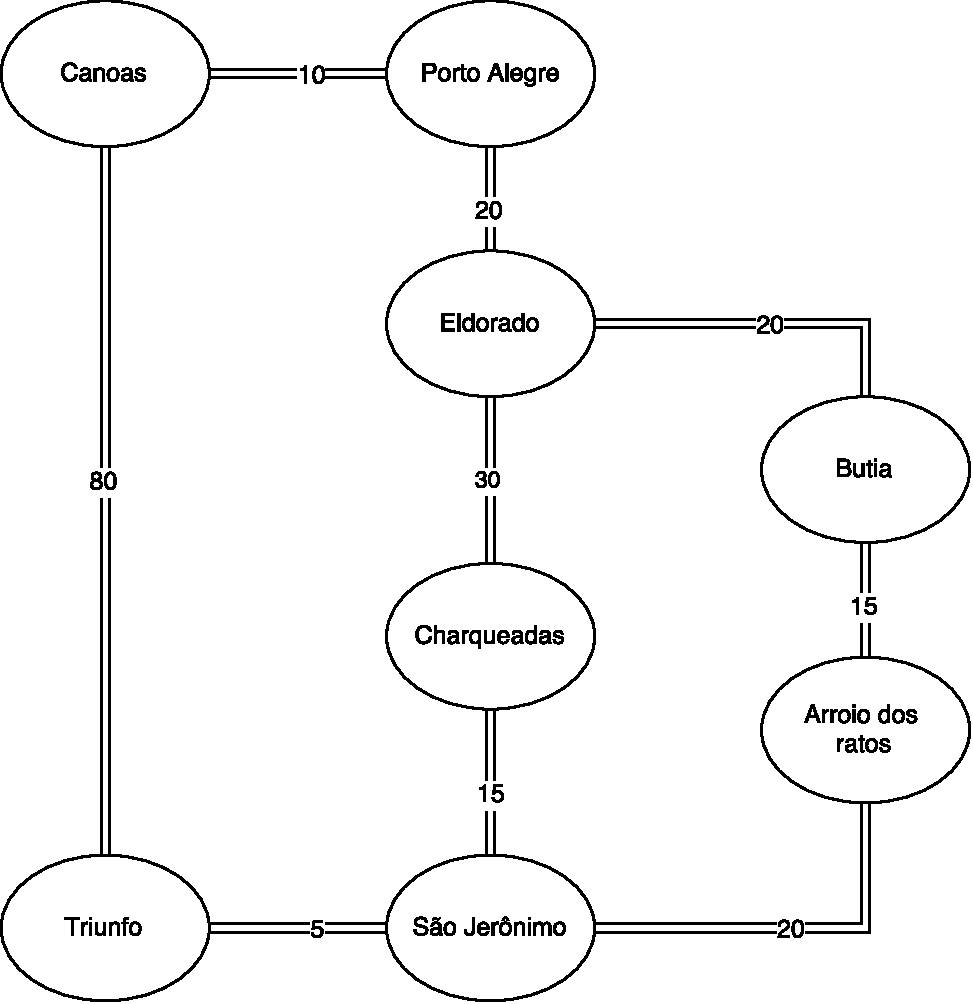
\includegraphics[width=0.6\textwidth]{fig/mapabusca.pdf}
	\caption{Mapa para o exemplo de problema de busca}
	\label{fig:mapabusca}
\end{figure} 

Para atingir o objetivo é preciso tentar os possíveis caminhos até o objetivo. 
Digamos que o agente comece sua viagem indo para a cidade de Triunfo, para nós (humanos) é intuitivo que a escolha não foi a melhor para iniciar, mas a técnica só tem como saber após realizar todas as possíveis opções de caminhos, ou se utilizar junto a técnica uma função de heurística, levando em consideração os custos dos caminhos, que acrescentam um conhecimento extra para a resolução do problema~\cite[Capítulo 3]{intelligence2003modern}.

\section{Busca adversária}

Jogos são difíceis de resolver com técnicas de IA, pois eles requerem a habilidade de tomar algum tipo de decisão, e as técnicas comuns as vezes não são satisfatórias, seja pelo fato do conjunto de estados possíveis de se atingir ser muito grande, ou pelo curto espaço de tempo para tomar essa decisão.
A busca adversaria pode ser utilizada nos jogos que estão situados em ambientes competitivos e de multi agentes.
Em um jogo, o jogador não informa suas jogadas previamente, mas está sempre buscando vencer o jogo, por essa razão é possível prever as suas ações.
No xadrez, os jogadores alternam jogadas até que um jogador ganha, e o outro perde. Uma maneira de representar uma vitória é atribuindo um valor de utilidade positivo para aquela configuração do jogo, e consequentemente um valor de utilidade negativo para uma derrota. Isto faz com que no final do jogo, quando os valores de utilidade dos agentes forem somados, a sua soma seja sempre zero. 
Com o intuito de resolver esse problema, é possível gerar uma solução de contingência para tentar antecipar as jogadas do adversário~\cite[Capítulo 5]{intelligence2003modern}. 

As técnicas de busca adversária utilizam uma variação da definição de um problema de busca comum. 
Os componentes sofrem algumas mudanças para se adequar ao ambiente competitivo.
Por esse motivo os componentes são redefinidos como:

\begin{itemize}
	\item $s_{0}$, sendo o estado inicial, que especifica como o jogo se configura no início;
	\item $players(s)$, define qual jogador tem o movimento no estado $s$;
	\item $actions(s)$, conjunto das ações possíveis em um estado $s$;
	\item $result(s, a)$, um modelo de transição, que define o resultado da ação $a$ a aplicada ao estado $s$;
	\item $terminal(s)$, verifica se o estado $s$ é um estado onde o jogo termina; e
	\item $utility(s,p)$, define um valor numérico, representando o lucro do jogador $p$ ao atingir o estado terminal $s$. Também é chamado de função de avaliação.
\end{itemize}

Com estes componentes descritos é possível formalizar o que é uma árvore de jogadas. 
A árvore de jogados, ou \textit{game tree}, contém os estados do jogo e os movimentos possíveis em cada estado. 
A \textit{game tree} é composta pelo estado inicial ($s_{0}$), as ações (\texttt{action(s)}) e o modelo de transição (\texttt{result(s, a)}), e possui uma profundidade ($d$), que indica o nível máximo da árvore. 
Cada nodo da árvore representa um estado do jogo. 
Os nodos tem uma ligação para cada ação possível. As ligações representam as ações, o nodo resultante da ligação é o novo estado do jogo após a execução da ação.
Um nodo folha é alcançado quando há uma configuração de fim de jogo.
Considerando o jogo de jogo da velha, onde cada jogador realiza uma jogada de cada vez, uma \textit{game tree} que mostra parte das jogadas do jogo da velha é ilustrada na Figura~\ref{fig:jogodavelha}. 
O estado inicial do jogo é o campo vazio, a cada nível da árvore todas as possibilidades de jogadas são testadas, a profundidade $d$ dessa árvore chega a 9 quando ela estiver completa, pois a cada nível da árvore uma jogada é marcada no campo. 

\begin{figure}[ht]
	\centering
	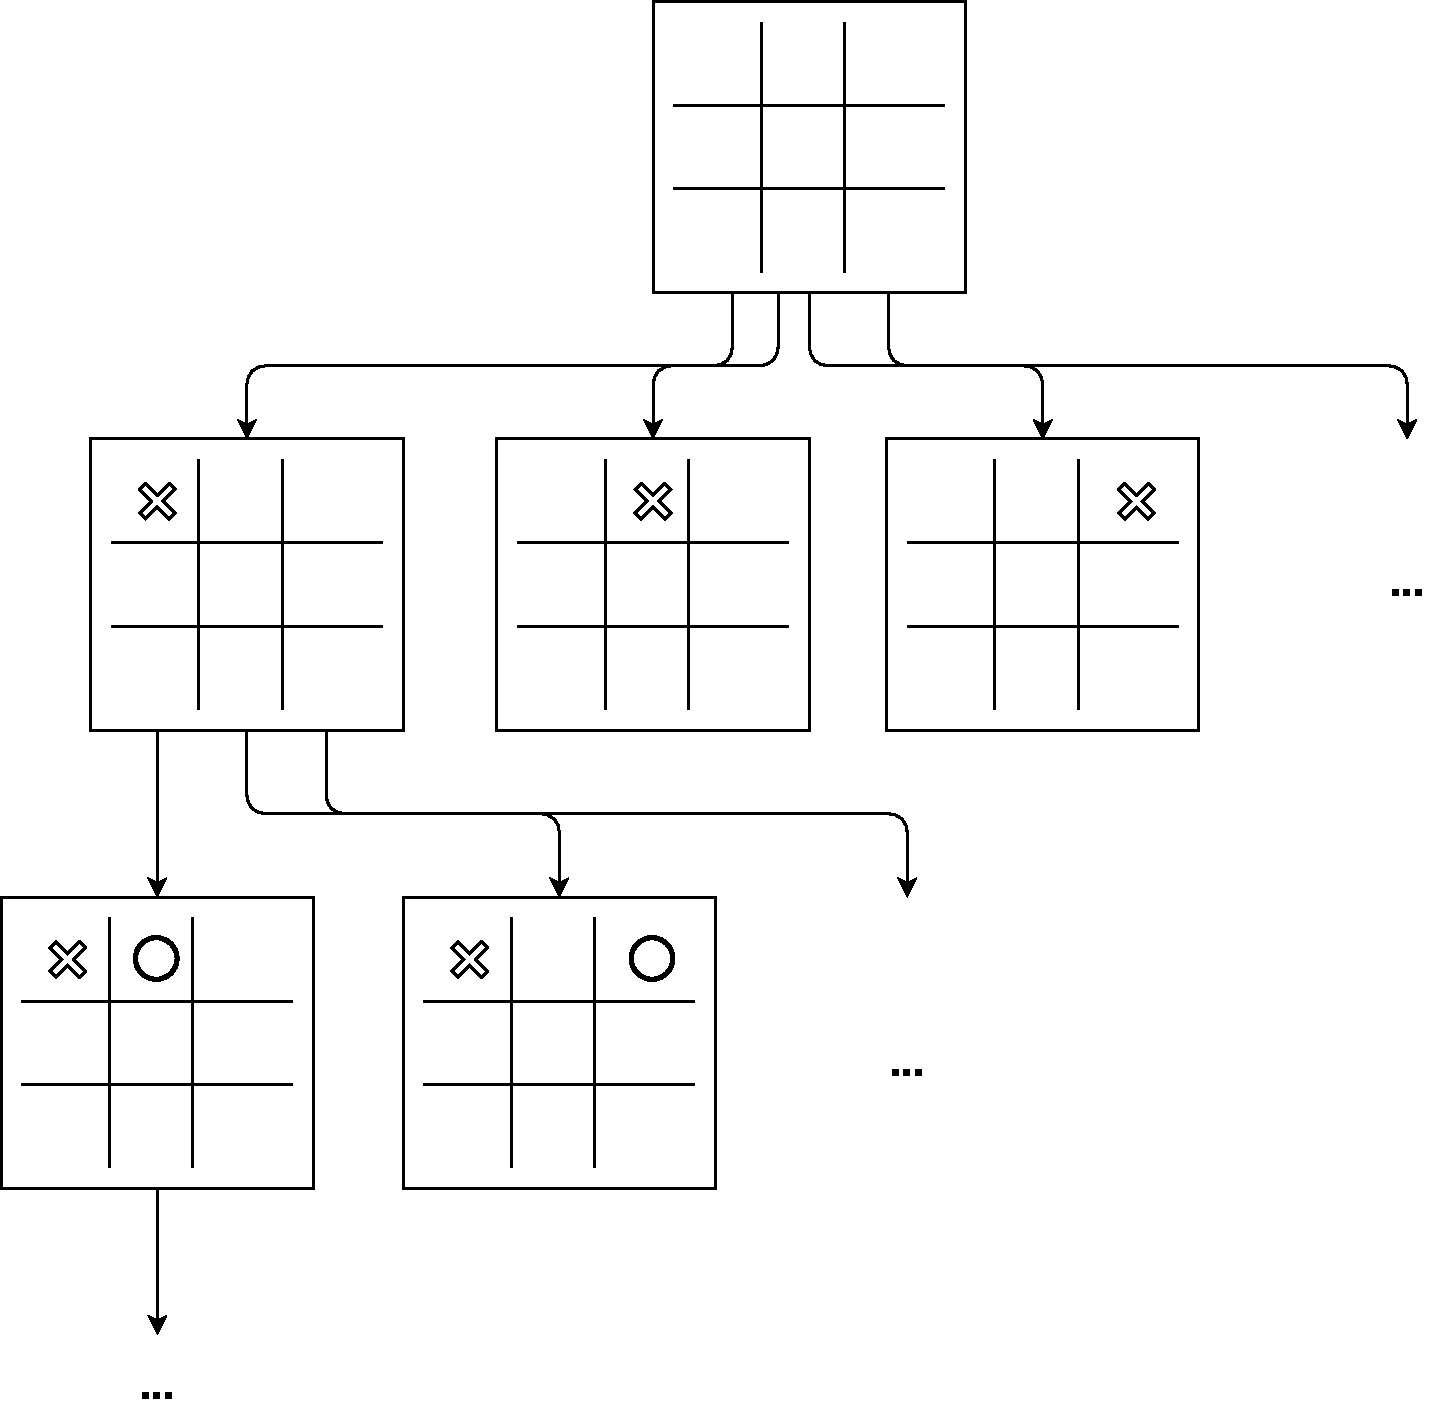
\includegraphics[width=0.5\textwidth]{fig/jogodavelha.pdf}
	\caption{Exemplo de um pedaço de uma \textit{game tree} sobre o jogo da velha}
	\label{fig:jogodavelha}
\end{figure} 

\section{Minimax search}
\label{sec:minimax}

O \textit{minimax search} é um algoritmo de busca adversária, seu objetivo é retornar a melhor jogada para o estado atual. 
Este método considera dois agentes, chamados de \textsc{Max} e \textsc{Min}, onde o jogador \textsc{Max} representa a perspectiva do agente que está tentando maximizar a recompensa de suas ações em relação ao agente \textsc{Min}, que representa o agente adversário do jogador \textsc{Max}. 
O algoritmo alterna entre jogadas de \textsc{Max}, e \textsc{Min}~\cite[Capítulo 5]{intelligence2003modern}. 

O algoritmo utiliza a \textit{game tree} para analisar todos os estados possíveis do jogo, e assim decidir qual a ação que quando aplicada ao seu estado atual, trará um melhor benefício no futuro, se caracterizando a melhor jogada. 
Os nodos folhas da árvore, que representam o final do jogo, contém um valor de utilidade, obtido pela função de avaliação. 
Os valores mais altos são as melhores jogadas para \textsc{Max}, e consequentemente, os valores menores são melhores para \textsc{Min}. 
Ao chegar no final da árvore, o algoritmo consegue o valor de utilidade para aquele cenário do jogo, quando isso acontece, o algoritmo faz o caminho inverso na árvore, analisando os outros possíveis cenários~\cite[Capítulo 5]{intelligence2003modern}. 
A Figura~\ref{fig:gametree} ilustra uma árvore de jogo, que simula o comportamento do algoritmo de \textit{minimax search}. Nessa árvore é possível observar que os nodos folhas contém o valor de utilidade para as configurações de final de jogo de cada estado, e nos nodos superiores é escolhida a jogada que minimiza as chances do jogador \textsc{Min} ganhar, e aumenta as chances do jogador \textsc{Max} ganhar.

\begin{figure}[ht]
	\centering
	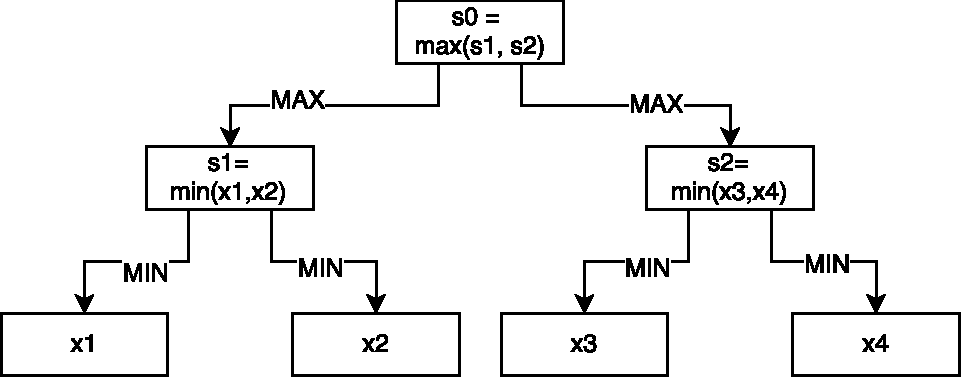
\includegraphics[width=0.6\textwidth]{fig/gametree.pdf}
	\caption{Exemplo de game tree utilizando \textit{minimax search}}
	\label{fig:gametree}
\end{figure} 

O método de \textit{minimax search} assume que todos os jogadores são racionais.
Com isso o algoritmo considera que os agentes sempre realizarão uma jogada para tentar ganhar o jogo.
O algoritmo de \textit{minimax search} é ilustrado no Algoritmo~\ref{alg:minimax}. 
O algoritmo tem como retorno a melhor ação a ser realizada no estado atual. 
As funções presentes nas linhas~\ref{alg:minimax:max} e ~\ref{alg:minimax:min} são utilizadas para calcular a jogada na visão de \textsc{Max} e \textsc{Min} respectivamente.
A função presente na linha~\ref{alg:minimax:minimax} é utilizada para iniciar a recursão e ao final retornar o melhor valor de utilidade para o jogador \textsc{Max}.

\begin{algorithm}
	\caption{Minimax Search}
	\label{alg:minimax}
	\begin{algorithmic}[1]	
		\Function{Minimax}{$state$} \label{alg:minimax:minimax}
		\State \Return $arg max_{action~ \in~ actions(s)}~ min\_value(result(state,  action)) $
		\EndFunction \\
		\Function {Max\_Value}{$state$}\label{alg:minimax:max}
		\If {$terminal(state)$}
		\State	\Return $utility(state)$
		\EndIf
		\State $v = -\infty$
		\ForAll{$action \in actions(state)$}
		\State $v = max(v, min\_value(result(state,action)))$
		\EndFor	
		\EndFunction \\
		\Function {Min\_Value}{$state$}\label{alg:minimax:min}
		\If {$terminal(state)$}
		\State	\Return $utility(state)$
		\EndIf
		\State $v = \infty$
		\ForAll{$action \in actions(state)$}
		\State $v = min(v, max\_value(result(state,action)))$
		\EndFor	
		\EndFunction
	\end{algorithmic}
\end{algorithm}


O algoritmo de \textit{minimax} deve explorar todo o espaço de estados para conseguir encontrar a ação que deve ser executada. 
A quantidade de estados possíveis, dependendo da situação, pode ser muito alta, no xadrez esse número chega a $10^{50}$, em um jogo de \textit{poker} no estilo \textit{texas holdem} esse número pode chegar a $10^{80}$. 
Geralmente, as ações devem ser tomadas em um curto período de tempo. 
Por esse motivo, utilizar técnicas de busca para jogos pode ser um problema. 
Existem algumas abordagens que utilizam busca adversaria com um nível de abstração mais alto para tentar minimax esse problema~\cite{ontanon2013survey}. Outras abordagens diminuem o espaço de estados, cortando caminhos que não influenciam no resultado final~\cite[Capítulo 5]{intelligence2003modern}